%%%%%%%%%%%%%%%%%%%%%%%%%%%%%%%%%%%%%
%                                   %
% Compile with XeLaTeX and biber    %
%                                   %
% Questions or comments:            %
%                                   %
% joshua dot mcneill at uga dot edu %
%                                   %
%%%%%%%%%%%%%%%%%%%%%%%%%%%%%%%%%%%%%

\documentclass{beamer}
  % Read in standard preamble (cosmetic stuff)
  %%%%%%%%%%%%%%%%%%%%%%%%%%%%%%%%%%%%%%%%%%%%%%%%%%%%%%%%%%%%%%%%
% This is a standard preamble used in for all slide documents. %
% It basically contains cosmetic settings.                     %
%                                                              %
% Joshua McNeill                                               %
% joshua dot mcneill at uga dot edu                            %
%%%%%%%%%%%%%%%%%%%%%%%%%%%%%%%%%%%%%%%%%%%%%%%%%%%%%%%%%%%%%%%%

% Beamer settings
% \usetheme{Berkeley}
\usetheme{CambridgeUS}
% \usecolortheme{dove}
% \usecolortheme{rose}
\usecolortheme{seagull}
\usefonttheme{professionalfonts}
\usefonttheme{serif}
\setbeamertemplate{bibliography item}{}

% Packages and settings
\usepackage{fontspec}
  \setmainfont{Charis SIL}
\usepackage{hyperref}
  \hypersetup{colorlinks=true,
              allcolors=blue}
\usepackage{graphicx}
  \graphicspath{{../../figures/}}
\usepackage[normalem]{ulem}
\usepackage{enumerate}

% Document information
\author{M. McNeill}
\title[FREN2001]{Français 2001}
\institute{\url{joshua.mcneill@uga.edu}}
\date{}

%% Custom commands
% Lexical items
\newcommand{\lexi}[1]{\textit{#1}}
% Gloss
\newcommand{\gloss}[1]{`#1'}
\newcommand{\tinygloss}[1]{{\tiny`#1'}}
% Orthographic representations
\newcommand{\orth}[1]{$\langle$#1$\rangle$}
% Utterances (pragmatics)
\newcommand{\uttr}[1]{`#1'}
% Sentences (pragmatics)
\newcommand{\sent}[1]{\textit{#1}}
% Base dir for definitions
\newcommand{\defs}{../definitions}


  % Packages and settings
  \usepackage{tikz}
  \usepackage[backend=biber, style=apa]{biblatex}
    \addbibresource{../references/References.bib}

  % Document information
  \subtitle[More Compositional Semantics]{More Compositional Semantics}

  %% Custom commands
  % Subsection/frame titles
  \newcommand{\suboneone}{Intuition}
  \newcommand{\subonetwo}{NP and VP combinations}
  \newcommand{\subonethree}{AP and N combinations}
  \newcommand{\subonefour}{Practice}

\begin{document}
  % Read in the standard intro slides (title page and table of contents)
  %%%%%%%%%%%%%%%%%%%%%%%%%%%%%%%%%%%%%%%%%%%%%%%%%%%%%%%%%%%%%%%%
% This is a standard set of intro slides used in for all slide %
% documents. It basically contains the title page and table of %
% contents.                                                    %
%                                                              %
% Joshua McNeill                                               %
% joshua dot mcneill at uga dot edu                            %
%%%%%%%%%%%%%%%%%%%%%%%%%%%%%%%%%%%%%%%%%%%%%%%%%%%%%%%%%%%%%%%%

\begin{frame}
  \titlepage
  \tiny{Office: % Basically a variable for office hours location
Gilbert 121\\
        Office hours: % Basically a variable for office hours
 lundi, mercredi, vendredi 10:10--11:10
}
\end{frame}

\begin{frame}
  \tableofcontents[hideallsubsections]
\end{frame}

\AtBeginSection[]{
  \begin{frame}
    \tableofcontents[currentsection,
                     hideallsubsections]
  \end{frame}
}


  \section{More Compositional Semantics}
    \subsection{\suboneone}
      \begin{frame}{\suboneone}
        \begin{block}{}
          So far we've used intuition to obtain truth values for propositions like:
          \begin{enumerate}
            \item The dog barks.
          \end{enumerate}
        \end{block}
        \begin{block}{}
          We can do better
        \end{block}
      \end{frame}

    \subsection{\subonetwo}
      \begin{frame}{\subonetwo}
        \begin{block}{`The dog barks'}
          \only<1>{
            True when the dog in question is part of the intersection of the NP's reference and the VP's reference
          }
          \only<2>{
            \small{
              $\text{TV}\left(\text{dog barking}\right) = \text{true} \iff \text{animal} \in \text{DOG} \land \text{action} \in \text{BARKING}$
            }
          }
        \end{block}
        \begin{center}
          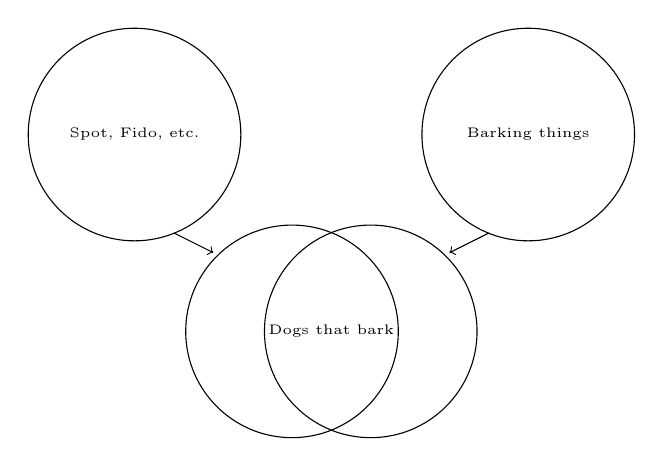
\begin{tikzpicture}
            \draw (0,0)  circle (1.35cm) node[font=\tiny] (dogsA)    {Spot, Fido, etc.};
            \draw (5,0)  circle (1.35cm) node[font=\tiny] (barkingA) {Barking things};
            \draw (2,-2.5) circle (1.35cm) node (dogsB)    {};
            \draw (3,-2.5) circle (1.35cm) node (barkingB) {};
            \draw[->] (0.5,-1.25) -- (1,-1.5);
            \draw[->] (4.5,-1.25) -- (4,-1.5);
            \path (dogsB) -- (barkingB) node[midway,font=\tiny] {Dogs that bark};
          \end{tikzpicture}
        \end{center}
      \end{frame}

    \subsection{\subonethree}
      \begin{frame}[t]{\subonethree}
        \begin{block}{`green sweater'}
          \begin{itemize}
            \item Some AP + N combinations work similarly
          \end{itemize}
        \end{block}
        \only<1>{
          \begin{center}
            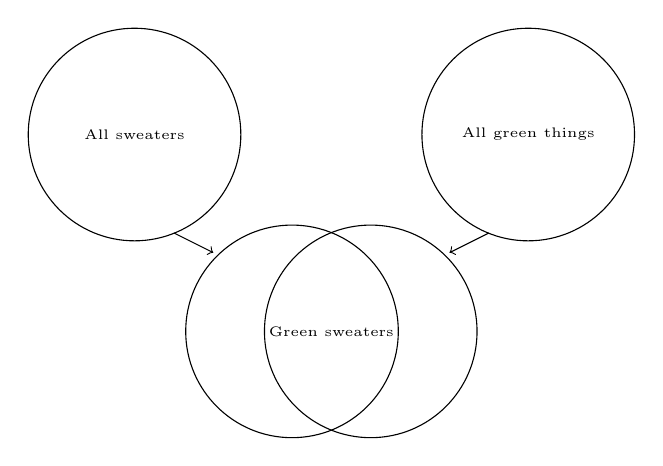
\begin{tikzpicture}
              \draw (0,0)  circle (1.35cm) node[font=\tiny] (sweatersA) {All sweaters};
              \draw (5,0)  circle (1.35cm) node[font=\tiny] (greenA)    {All green things};
              \draw (2,-2.5) circle (1.35cm) node (sweatersB) {};
              \draw (3,-2.5) circle (1.35cm) node (greenB)    {};
              \draw[->] (0.5,-1.25) -- (1,-1.5);
              \draw[->] (4.5,-1.25) -- (4,-1.5);
              \path (sweatersB) -- (greenB) node[midway,font=\tiny] {Green sweaters};
            \end{tikzpicture}
          \end{center}
        }
        \only<2->{
          \begin{alertblock}{Pure intersective adjectives}
            % Pure intersective adjective
An adjective whose set of referents can be understood independently of the set of referents of the noun

          \end{alertblock}
        }
      \end{frame}

      \begin{frame}{\subonethree}
        \begin{block}{Semantic types of adjectives}
          \begin{itemize}
            \item Intersective adjectives
            \begin{itemize}
              \item Pure intersective adjectives
              \item Subsective adjectives
            \end{itemize}
            \item Non-intersective adjectives
            \begin{itemize}
              \item Anti-intersective adjectives
            \end{itemize}
          \end{itemize}
        \end{block}
      \end{frame}

      \begin{frame}{\subonethree}
        \begin{alertblock}{Subsective adjectives}
          % Subsective adjective
An adjective whose set of referents cannot be understood independently of the set of referents of the noun

        \end{alertblock}
        \begin{block}{`big mouse', `big whale'}
          The AP can't be understood independently of the N
        \end{block}
        \begin{center}
          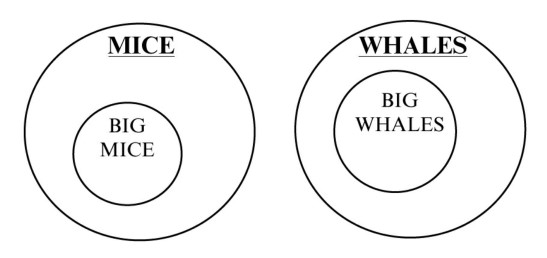
\includegraphics[scale=0.75]{big.jpg}
        \end{center}
      \end{frame}

      \begin{frame}{\subonethree}
        \begin{alertblock}{Non-intersective adjectives}
          % Non-intersective adjective
An adjective which, when combined with a noun, indicates a set of referents that may or may not be included in the set of referents of the noun alone

        \end{alertblock}
        \begin{example}
          \begin{enumerate}
            \item possible solution
            \item alleged thief
          \end{enumerate}
        \end{example}
      \end{frame}

      \begin{frame}{\subonethree}
        \begin{alertblock}{Anti-intersective adjectives}
          % Anti-intersective adjective
An adjective which, when combined with a noun, indicates a set of referents that are definitely not included in the set of referents of the noun alone

        \end{alertblock}
        \begin{example}
          \begin{enumerate}
            \setcounter{enumi}{2}
            \item fake Picasso
            \item counterfeit dollar
          \end{enumerate}
        \end{example}
      \end{frame}

    \subsection{\subonefour}
      \begin{frame}{\subonefour}
        \begin{block}{Try these}
          \textcite{dawson_language_2016}, chapter 6 exercise 29
        \end{block}
      \end{frame}

\end{document}
